%%%%%%%%%%%%%%%%%%%%%%%%%%%%%%%%%%%%%%%%%
% Short Sectioned Assignment
% LaTeX Template
% Version 1.0 (5/5/12)
%
% This template has been downloaded from:
% http://www.LaTeXTemplates.com
%
% Original author:
% Frits Wenneker (http://www.howtotex.com)
%
% License:
% CC BY-NC-SA 3.0 (http://creativecommons.org/licenses/by-nc-sa/3.0/)
%
%%%%%%%%%%%%%%%%%%%%%%%%%%%%%%%%%%%%%%%%%

%----------------------------------------------------------------------------------------
%	PACKAGES AND OTHER DOCUMENT CONFIGURATIONS
%----------------------------------------------------------------------------------------

\documentclass[paper=a4, fontsize=11pt]{scrartcl} % A4 paper and 11pt font size

\usepackage{fourier} % Use the Adobe Utopia font for the document - comment this line to return to the LaTeX default
\usepackage[french]{babel} % English language/hyphenation
\usepackage{amsmath,amsfonts,amsthm} % Math packages

\usepackage{lipsum} % Used for inserting dummy 'Lorem ipsum' text into the template
\usepackage{graphicx}
\usepackage{sectsty} % Allows customizing section commands
\allsectionsfont{\centering \normalfont\scshape} % Make all sections centered, the default font and small caps

% tentative pour les algorithmes 
\usepackage{algorithm}
\usepackage{algpseudocode}

\usepackage{fancyhdr} % Custom headers and footers
\pagestyle{fancyplain} % Makes all pages in the document conform to the custom headers and footers
\fancyhead{} % No page header - if you want one, create it in the same way as the footers below
\fancyfoot[L]{} % Empty left footer
\fancyfoot[C]{} % Empty center footer
\fancyfoot[R]{\thepage} % Page numbering for right footer
\renewcommand{\headrulewidth}{0pt} % Remove header underlines
\renewcommand{\footrulewidth}{0pt} % Remove footer underlines
\setlength{\headheight}{13.6pt} % Customize the height of the header

\numberwithin{equation}{section} % Number equations within sections (i.e. 1.1, 1.2, 2.1, 2.2 instead of 1, 2, 3, 4)
\numberwithin{figure}{section} % Number figures within sections (i.e. 1.1, 1.2, 2.1, 2.2 instead of 1, 2, 3, 4)
\numberwithin{table}{section} % Number tables within sections (i.e. 1.1, 1.2, 2.1, 2.2 instead of 1, 2, 3, 4)

\setlength\parindent{0pt} % Removes all indentation from paragraphs - comment this line for an assignment with lots of text

%----------------------------------------------------------------------------------------
%	TITLE SECTION
%----------------------------------------------------------------------------------------

\newcommand{\horrule}[1]{\rule{\linewidth}{#1}} % Create horizontal rule command with 1 argument of height

\title{	
\normalfont \normalsize 
\textsc{Ecole Centrale de Nantes} \\ [25pt] % Your university, school and/or department name(s)
\horrule{0.5pt} \\[0.4cm] % Thin top horizontal rule
\huge Option Informatique - Corrigé TD MADIS \\ % The assignment title
\horrule{2pt} \\[0.5cm] % Thick bottom horizontal rule
}

%\author{Durée 1h - Aucun document autorisé} % Your name

%\date{\normalsize\today} % Today's date or a custom date

\begin{document}

\maketitle % Print the title

\section{L'itinéraire de Michel Strogoff}

\subsection{Itinéraire}

Dans cette première partie, on va appliquer une version légèrement modifiée de l'algorithme de Ford-Bellman. C'est possible car notre graphe ne comporte pas de boucles, cf figure~\ref{fig:ms}.

\begin{figure}[htbp]
\begin{center}
	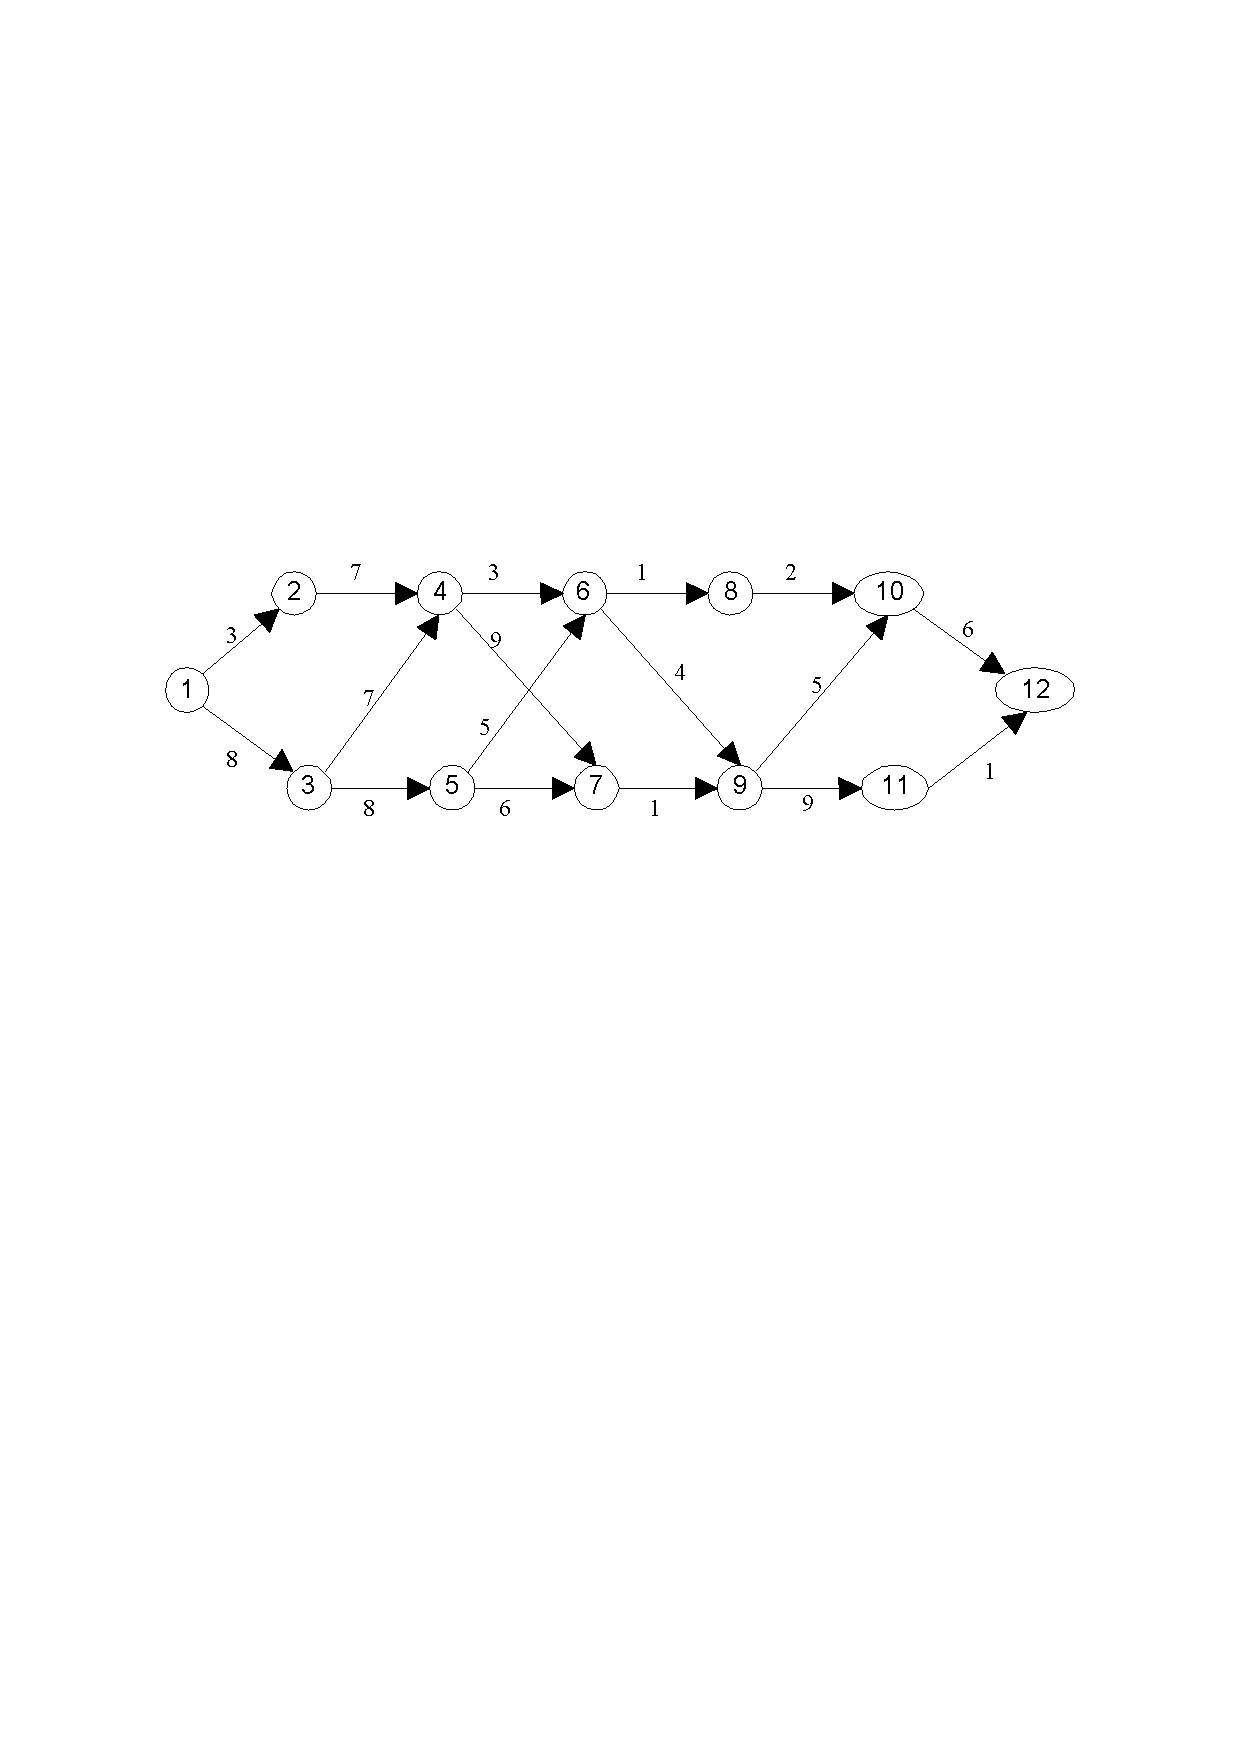
\includegraphics[width=.8\textwidth]{strogoff.pdf}
	\caption{Itinéraires possibles et chances de succès pour un trajet d'une ville à l'autre}
	\label{fig:ms}
\end{center}
\end{figure}

La seule modification à apporter à l'algorithme ordinal consiste à remplacer le min par un max. 


\begin{table}[htbp]
  \begin{center}
    \begin{tabular}{cccccccccccc}
      \hline
      $\epsilon$ & 1 & 1 & 3 & 3 & 5 & 4 & 6 & 6,7 & 9 & 9 & 10 \\
      \hline
      1 & 2 & 3 & 4 & 5 & 6 & 7 & 8 & 9 & 10 & 11 & 12 \\
      \hline
      0  \\
      0 & 3  \\
      0 & 3 & 8 \\
      0 & 3 & 8 & 15 \\
      0 & 3 & 8 & 15 & 16\\
      0 & 3 & 8 & 15 & 16 & 21 \\
      0 & 3 & 8 & 15 & 16 & 21 & 24\\
      0 & 3 & 8 & 15 & 16 & 21 & 24 & 22 \\
      0 & 3 & 8 & 15 & 16 & 21 & 24 & 22 & 25 \\
      0 & 3 & 8 & 15 & 16 & 21 & 24 & 22 & 25 & 30 \\
      0 & 3 & 8 & 15 & 16 & 21 & 24 & 22 & 25 & 30 & 34 \\
      0 & 3 & 8 & 15 & 16 & 21 & 24 & 24 & 25 & 30 & 34 & 36 \\
    \end{tabular}
  \end{center}
  \caption{Tableau des itérations de l'algorithme}
  \label{tab:fb}
\end{table}

Si on remonte à partir du sommet 12, on obtient deux chemins de longueur équivalente :
\begin{itemize}
\item 12-10-9-6-5-3-1
\item 12-10-9-7-4-3-1
\end{itemize}

\subsection{Probabilité de succès}

Ici, on se contente de considérer que $x$ chances sur $10$ de succès constituent une probabilité de $\frac{x}{10}$ de succès et que toutes les variables sont indépendantes. 

Dans le premier cas, nous obtenons alors une probabilité $p_1=0.0384$, tandis que pour le second, nous avons $p_2 = 0.01512$, ce qui est sensiblement moins bon. 

\subsection{Avec calcul des probabilités}

Toujours sous réserve de l'hypothèse des variables indépendantes, il faudrait passer au log pour considérer ensuite des multiplications de probabilités. L'algorithme de Ford-Bellman s'adapte alors facilement en faisant attention aux inversions de signe.


\section{Voyages aériens}

Une compagnie aérienne dessert différentes villes européennes. Le tableau~\ref{gr:airtravel} reprend les durées des vols entre ces différentes villes. 

\begin{table}[htbp]
\begin{center}

\begin{tabular}{|c|c|c|c|c|c|}
\hline 
 & \textbf{A}  & \textbf{B} & \textbf{C} & \textbf{D} & \textbf{E} \\ 
\hline 
\textbf{A} &  & 1h30  & 2h &  & 2h15 \\ 
\hline 
\textbf{B} & 1h40 &  &  &  & 3h \\ 
\hline 
\textbf{C} & 2h20 &  &  & 2h55 &  \\ 
\hline 
\textbf{D} &  & 3h20 &  &  & 1h05 \\ 
\hline 
\textbf{E} & 2h25 & 3h10 & 1h10 &  &  \\ 
\hline 
\end{tabular} 
\caption{Temps de vol entre les différentes villes}
\label{gr:airtravel}
\end{center}
\end{table}

\begin{enumerate}
\item Quels sont les plus courts trajets entre les différentes villes ? Quel est l'algorithme à utiliser et pourquoi ?
\item Comment modifier la méthode précédente pour tenir compte du temps d'escale dans chaque ville ? 
\end{enumerate}
\section{Débit réseau}

On s'intéresse maintenant à un problème de réseau. Pour une visio-conférence, on doit envoyer des paquets de données d'un point A vers un point B. TCP/IP permettant un routage des paquets, les paquets de données peuvent circuler sur différentes connexions avec un débit différent. On fera l'hypothèse que les paquets arrivent en ordre. 

\begin{figure}[htbp]
\begin{center}
	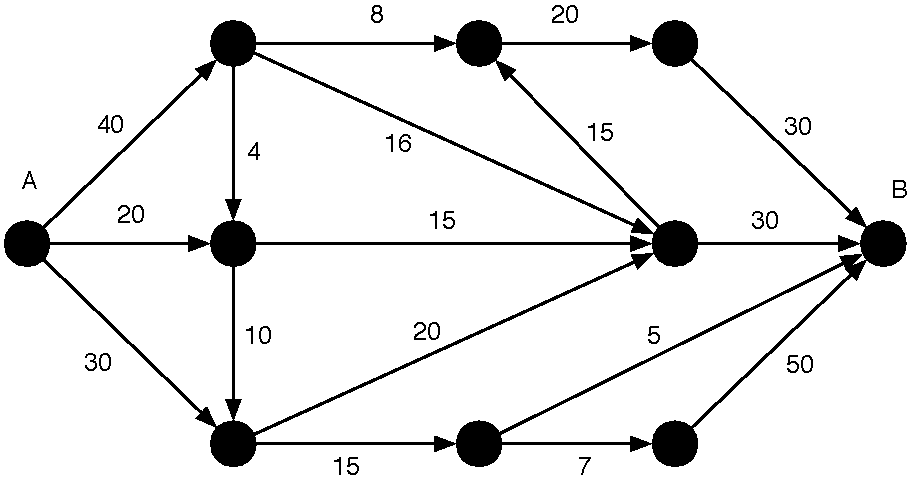
\includegraphics[width=.8\textwidth]{graphe1.pdf}
\end{center}
\end{figure}

\begin{enumerate}
\item Calculer le débit maximum atteignable avec le réseau de la figure précédente.
\item Quelle est la première liaison dont il faut augmenter le débit pour augmenter le débit global ?
\end{enumerate}
\section{Acheminement de passagers}

Lors de la mise en place d'un voyage organisé, un vol charter est
prévu au départ d'une ville F, un samedi soir. Les participants à ce
vol viennent de trois villes A, B et C avec des possibilités limitées
d'acheminement de ces villes jusqu'à F. Des départs sont prévus au
départ de A, B et C les jeudi, vendredi et samedi matins. Les
destinations possibles et le nombre de places disponibles sont
indiquées dans le tableau~\ref{tab:vol}.

\begin{table}[htbp]
  \begin{center}
    \begin{tabular}{|l|ccccc|}
      \hline
      & A vers B & A vers F & B vers C & B vers F & C vers F \\
     \hline 
      jeudi matin & 10 & 20 & 30 & 30 & 20 \\
      vendredi matin & 10 & 20 & 30 & 20 & 20 \\
      samedi matin & 0 & 25 & 0 & 65 & 40 \\
      \hline
    \end{tabular}
    \caption{Capacités de transport}
    \label{tab:vol}
  \end{center}
\end{table}

Pour chacun des départs, l'arrivée a lieu le soir même. Il est
possible de prévoir des transits et de passer une ou plusieurs nuits
dans chacune des villes, en fonction des capacités d'hébergement
répertoriées dans le tableau~\ref{tab:nuit}.

\begin{table}[htbp]
  \begin{center}
    \begin{tabular}{|l|cccc|}
      \hline
      & A & B & C & F \\
      \hline
      nuit de jeudi à vendredi & 30 & 50 & 40 & 25 \\
      nuit de vendredi à samedi & 15 & 55 & 40 & 40 \\
      \hline
    \end{tabular}
    \caption{Capacités d'accueil}
    \label{tab:nuit}
  \end{center}
\end{table}

Le nombre de personnes pouvant rester dans une ville durant la journée
n'est pas limité. Tous les participants du voyage doivent être pris en
charge à partir du jeudi matin (transport et hébergement). Il y a une
limitation a priori sur le nombre d'inscriptions (100 participants au
départ de A, autant de B et C). 

On cherche à acheminer le plus de participants possibles pour le vol
charter en tenant compte de ces contraintes.

\begin{enumerate}
\item définir un réseau de transport avec capacités permettant de
   formaliser le problème comme un problème de flot
   maximal. (indication : pour chaque ville $\alpha$, considérer deux
   sommets $\alpha_i$ et $\alpha_i'$ correspondant respectivement au
   matin et au soir du jour $j$).

\item résoudre le problème. combien de participants issus de A
   (respectivement B et C) pourront bénéficier du vol charter, selon
   la solution trouvée ?
\end{enumerate}


\end{document}
%%% Local Variables: 
%%% mode: latex
%%% TeX-master: t
%%% End: 
